\documentclass[submit]{harvardml}


\course{CS181-S24}
\assignment{Assignment \#1}
\duedate{11:59pm ET, February 10, 2024} 

\usepackage[OT1]{fontenc}
\usepackage[colorlinks,citecolor=blue,urlcolor=blue]{hyperref}
\usepackage[pdftex]{graphicx}
\usepackage{graphicx}
\usepackage{caption}
\usepackage{fullpage}
\usepackage{enumitem}
\usepackage{soul}
\usepackage{amsmath}
\usepackage{amssymb}
\usepackage{color}
\usepackage{todonotes}
\usepackage{listings}
\usepackage{common}
\usepackage{framed}
\usepackage{float}
\usepackage{ifthen}

\usepackage[mmddyyyy,hhmmss]{datetime}

% Solution environment
\newenvironment{solution}
  {\color{blue}\section*{Solution}}
{}

\definecolor{verbgray}{gray}{0.9}

\lstnewenvironment{csv}{
  \lstset{backgroundcolor=\color{verbgray},
  frame=single,
  framerule=0pt,
  basicstyle=\ttfamily,
  columns=fullflexible}}{}

 \DeclareMathOperator*{\limover}{\overline{lim}}


\begin{document}
\begin{center}
{\Large Homework 1: Regression}\\
\end{center}

\subsection*{Introduction}
This homework is on different three different forms of regression:
kernelized regression, nearest neighbors regression, and linear
regression.  We will discuss implementation and examine their
tradeoffs by implementing them on the same dataset, which consists of
temperature over the past 800,000 years taken from ice core samples.

The folder \verb|data| contains the data you will use for this
problem. There are two files:
\begin{itemize}
    \item \verb|earth_temperature_sampled_train.csv| 
    \item \verb|earth_temperature_sampled_test.csv|
\end{itemize} 

Each has two columns.  The first column is the age of the ice core
sample.  The second column is the approximate difference in a year's temperature (K) 
from the average temperature of the 1,000 years preceding it. The temperatures were retrieved from ice cores in
Antarctica (Jouzel et al. 2007)\footnote{Retrieved from
\url{https://www.ncei.noaa.gov/pub/data/paleo/icecore/antarctica/epica_domec/edc3deuttemp2007.txt}

Jouzel, J., Masson-Delmotte, V., Cattani, O., Dreyfus, G., Falourd, 
S., Hoffmann, G., … Wolff, E. W. (2007). Orbital and Millennial 
Antarctic Climate Variability over the Past 800,000 Years. 
\emph{Science, 317}(5839), 793–796. doi:10.1126/science.1141038}.
 
The following is a snippet of the data file:
 
\begin{csv}
# Age, Temperature
399946,0.51
409980,1.57
\end{csv}

\noindent And this is a visualization of the full dataset: 
\begin{center}
  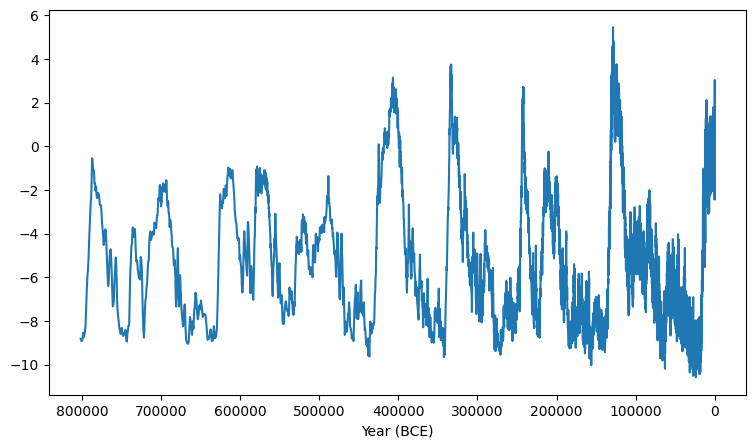
\includegraphics[width=.8\textwidth]{images/sample_graph}
    \end{center}
  \noindent 


\textbf{Due to the large magnitude of the years, we will work in terms
  of thousands of years BCE in Problems 1-3.} This is taken care of
for you in the provided notebook.






\subsection*{Resources and Submission Instructions}
If you find that you are having trouble with the first couple
problems, we recommend going over the fundamentals of linear algebra
and matrix calculus (see links on website).  The relevant parts of the
\href{https://github.com/harvard-ml-courses/cs181-textbook/blob/master/Textbook.pdf}{cs181-textbook
  notes are Sections 2.1 - 2.7}.  We strongly recommend reading the
textbook before beginning the homework.

We also encourage you to first read the
\href{http://users.isr.ist.utl.pt/~wurmd/Livros/school/Bishop\%20-\%20Pattern\%20Recognition\%20And\%20Machine\%20Learning\%20-\%20Springer\%20\%202006.pdf}{Bishop
  textbook}, particularly: Section 2.3 (Properties of Gaussian
Distributions), Section 3.1 (Linear Basis Regression), and Section 3.3
(Bayesian Linear Regression). (Note that our notation is slightly
different but the underlying mathematics remains the same!).

\textbf{Please type your solutions after the corresponding problems
  using this \LaTeX\ template, and start each problem on a new page.}
You may find the following introductory resources on \LaTeX\ useful:
\href{http://www.mjdenny.com/workshops/LaTeX_Intro.pdf}{\LaTeX\ Basics}
and
\href{https://www.overleaf.com/learn/latex/Free_online_introduction_to_LaTeX_(part_1)}{\LaTeX\ tutorial
  with exercises in Overleaf}

Homeworks will be submitted through Gradescope. You will be added to
the course Gradescope once you join the course Canvas page. If you
haven't received an invitation, contact the course staff through Ed.

\textbf{Please submit the writeup PDF to the Gradescope assignment
  `HW1'.} Remember to assign pages for each question.

\textbf{Please submit your \LaTeX file and code files to the
  Gradescope assignment `HW1 - Supplemental'.} Your files should be
named in the same way as we provide them in the repository,
e.g. \texttt{hw1.pdf}, etc.


%%%%%%%%%%%%%%%%%%%%%%%%%%%%%%%%%%%%%%%%%%%%%
% Problem 1
%%%%%%%%%%%%%%%%%%%%%%%%%%%%%%%%%%%%%%%%%%%%%
\newpage

\begin{problem}[Setting up the Regression, 10pts]
As noted in the introduction, your goal is to predict temperature
variation given the year.  Before we start deriving and coding up our
regressions, we will interrogate the set-up of our problem.  

\begin{enumerate}
  \item These data were derived from ice core samples in Antarctica.
    Take a brief look at the
    \href{https://www.ncei.noaa.gov/pub/data/paleo/icecore/antarctica/epica_domec/edc3deuttemp2007.txt}{original
      data file}.  Briefly discuss how the data were processed: what kinds of
    decisions and corrections had to be made?  We know that different
    places on earth have different temperatures: what does the
    temperature in the temperature column correspond to?
        
  \item Even before doing any formal regressions, we see that there is
    some periodicity in the data: there are years that are warmer, and
    years that are cooler.  Suppose you are a government official
    advising on how much to worry about climate change.  Would it be
    reasonable to use this pattern as evidence that the earth will
    cool down again?  Why or why not, or to what extent?


  \item In the problems below, we will focus on interpolating
    temperatures for years not provided in the training set.  What
    kind of application would such a regression be useful for?

\end{enumerate}
  
\end{problem}

% qwer
\begin{solution}

\textbf{1.}

The original data from the EPICA Dome C provides detailed deuterium profiles and temperature estimates, which were derived from ice core samples extending back approximately 800,000 years.\\

The data processing involve corrections for seawater isotopic composition and ice sheet elevation to estimate temperature differences from the average of the last 1000 years. This included calibrating raw isotopic measurements to reflect past temperatures, accounting for geographic and environmental changes over time, and possibly interpolating or smoothing data to handle gaps or anomalies. This shows that to prepare the sampled data, decisions about how to adjust for these environmental factors and the age model were necessary. The temperature in the temperature column corresponds to estimated differences in annual temperatures from a 1000-year average, and this reflects broader climatic changes rather than localized weather patterns. The temperature values represent anomalies relative to a baseline, likely involving models to adjust for various factors like changes in Earth's orbit or volcanic activity.

\bigskip
\textbf{2.}

Using the periodicity observed in ancient climate data to argue that the Earth will naturally cool again after a warming phase is misleading when discussing current climate change. It is true that Earth's climate has experienced natural fluctuations over millennia due to various factors like volcanic activity, solar radiation changes, and Earth's orbital variations. However, the rapid rate of current global warming, largely attributed to human activities like burning fossil fuels, deforestation, etc is unprecedented in this historical context. Relying solely on past climate cycles to predict future cooling ignores the impact of anthropogenic greenhouse gas emissions, which have significantly changed the Earth's energy balance.

\bigskip
\textbf{3.}

Interpolating temperatures for years not in the training set is particularly useful for reconstructing historical climate patterns, help us understand climate variability and trends over time. This can inform climate models, improve predictions of future climate scenarios, and guide policy and decision-making related to climate change adaptation and mitigation. It also can help scientists understand the impact of past climatic events on biodiversity, ecosystems etc.

\end{solution}
% rewq

%%%%%%%%%%%%%%%%%%%%%%%%%%%%%%%%%%%%%%%%%%%%%
% Problem 2
%%%%%%%%%%%%%%%%%%%%%%%%%%%%%%%%%%%%%%%%%%%%%

\begin{problem}[Optimizing a Kernel, 30pts]
Kernel-based regression techniques are similar to nearest-neighbor
regressors: rather than fit a parametric model, they predict values
for new data points by interpolating values from existing points in
the training set.  In this problem, we will consider a kernel-based
regressor of the form:
\begin{equation*}
  f_\tau(x^*) = \cfrac{\sum_{n} K_\tau(x_n,x^*) y_n}{\sum_n K_\tau(x_n, x^*)} 
\end{equation*}
where $\mathcal{D}_\texttt{train} = \{(x_n,y_n)\}_{n = 1} ^N$ are the
training data points, and $x^*$ is the point for which you want to
make the prediction.  The kernel $K_\tau(x,x')$ is a function that
defines the similarity between two inputs $x$ and $x'$. A popular
choice of kernel is a function that decays as the distance between the
two points increases, such as
\begin{equation*}
  K_\tau(x,x') = \exp\left\{-\frac{(x-x')^2}{\tau}\right\}
\end{equation*}
where $\tau$ represents the square of the lengthscale (a scalar value that 
dictates how quickly the kernel decays).  In this
problem, we will consider optimizing what that (squared) lengthscale
should be.

\noindent\emph{Make sure to include all required plots in your PDF.}

\begin{enumerate}
  
\item Let's first take a look at the behavior of the fitted model for different values of $\tau$. Implement the \texttt{kernel\_regressor} function in the notebook, and plot your model for years in the range $800,000$ BC to $400,000$ BC at $1000$ year intervals for the following three values of $\tau$: $1, 50, 2500$. Since we're working in terms of thousands of years, this means you should plot $(x, f_\tau(x))$ for $x = 400, 401, \dots, 800$. \textbf{The plotting has been set up} for you in the notebook already.

Include your plot in your solution PDF.

\textbf{In no more than 5 sentences}, describe how the fits change with $\tau$.

\item Now, we will evaluate the quality of each model \emph{quantitatively} by computing the error on some test set $\mathcal{D}_\texttt{test} = \{(x'_m, y'_m)\}_{m = 1} ^M$.  Write down the expression for MSE of $f_\tau$ over the test set as a function of the training set and test set. Your answer may include $\{(x'_m, y'_m)\}_{m = 1} ^M$, $\{(x_n, y_n)\}_{n = 1} ^N$, and $K_\tau$, but not $f_\tau$.

\item Suppose we used the training set as our test set, that is, we evaluated the expression above with $\mathcal{D}_\texttt{test} = \mathcal{D}_\texttt{train}$, and chose the value of $\tau$ which gave the smallest loss.  What value of $\tau$ would be picked?  Why is setting $\mathcal{D}_\texttt{test} = \mathcal{D}_\texttt{train}$ a bad idea?
   
\emph{Hint: consider what value of $\tau$ would be optimal, for $\tau$ ranging in $(0, \infty)$. We can consider $f_\tau(x^*)$ as a weighted average of the training responses, where the weights are proportional to the distance to $x^*$, and the distance is computed via the kernel. What happens to $K_\tau(x, x')$ as $\tau$ becomes very small, when $x = x'$? What about when $x \neq x'$?}

\item Let us compute the MSE on the provided test set (that is, not the training set). Write Python code to compute the MSE with respect to the same lengthscales as in Part 1. Which model yields the lowest test set MSE? 

\item Describe the time and space complexity of kernelized regression with respect to the size of the training set $N$.  How, if at all, does the size of the model---everything that needs to be stored to make predictions---change with the size of the training set $N$?  How, if at all, do the number of computations required to make a prediction for some input $x^*$ change with the size of the training set $N$?

\end{enumerate}

\end{problem}


% qwer
\begin{solution}

\textbf{1.}

\begin{figure}[h]
    \centering
    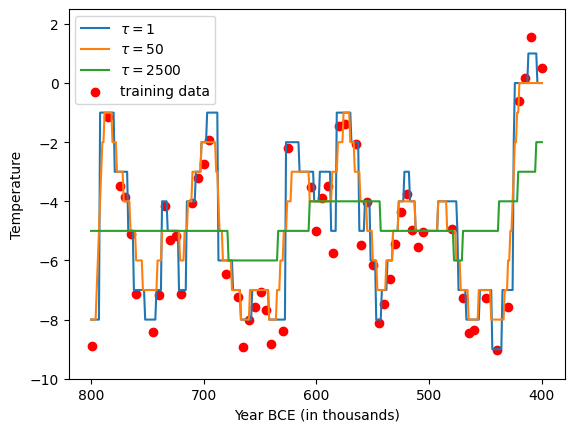
\includegraphics[width=0.5\linewidth]{image.png}
    \caption{Resulting plot}
    \label{fig:enter-label}
\end{figure}

For \(\tau = 1\), the fit is highly sensitive to the training data points, resulting in a jagged and fluctuating prediction line. This indicates a model that closely follows every up and down in the training set, leading to high variance and potential overfitting.\\

With \(\tau = 50\), the prediction curve becomes smoother, indicating a more generalized model that balances fitting to the data while avoiding overfitting to individual data points.\\

For \(\tau = 2500\), the model is very smooth, with predictions that show only the broadest trends in the data. This level of smoothness suggests a high-bias model that may underfit the data though.

\bigskip
\textbf{2.}

For the kernel-based regressor, the MSE over the test set can be expressed as below:

$$
\text{MSE} = \frac{1}{M} \sum_{m=1}^M \left(f_\tau(x_m') - y_m'\right)^2
$$

Given the definition of \(f_\tau(x^*)\) as

$$
f_\tau\left(x^*\right)=\frac{\sum_n K_\tau\left(x_n, x^*\right) y_n}{\sum_n K_\tau\left(x_n, x^*\right)}
$$

We can substitute \(f_\tau(x_m')\) in the MSE formula to get the expression for MSE in terms of the training set \(\left\{\left(x_n, y_n\right)\right\}_{n=1}^N\), the test set \(\left\{\left(x_m', y_m'\right)\right\}_{m=1}^M\), and the kernel function \(K_\tau\):

$$
\text{MSE} = \frac{1}{M} \sum_{m=1}^M \left(\frac{\sum_n K_\tau\left(x_n, x_m'\right) y_n}{\sum_n K_\tau\left(x_n, x_m'\right)} - y_m'\right)^2
$$

\bigskip
\textbf{3.}

When the training set is used as the test set, and we evaluate the expression for MSE with the aim of choosing the value of \(\tau\) that minimizes the loss, the chosen value of \(\tau\) would tend towards a very small number, approaching zero. This is because, as \(\tau\) becomes very small, the kernel \(K_\tau(x, x')\) becomes extremely sensitive to the distance between \(x\) and \(x'\).\\

For \(x = x'\), \(K_\tau(x, x')\) approaches 1 as \(\tau\) approaches 0 because the exponent \(\exp\left\{-\frac{(x-x')^2}{\tau}\right\}\) approaches \(\exp\{0\} = 1\). This means that the weight of the point itself becomes quite large compared to other points, making the prediction \(f_\tau(x^*)\) very close to the actual value \(y\) for the training points. The model becomes good at predicting the training data because it's essentially just memorizing the whole dataset. \\

For \(x \neq x'\), as \(\tau\) becomes very small, \(K_\tau(x, x')\) approaches 0, meaning that points even slightly distant from \(x^*\) have virtually no influence on the prediction. This results in a model that is highly overfitted to the training data, capturing noise in the training set as if it were a genuine pattern.\\

Choosing \(\tau\) in this way is a bad idea because it leads to overfitting. The model will perform exceptionally well on the training data but will likely perform poorly on unseen data because it has learned the noise and specific patterns of the training set rather than generalizable patterns. It gives an overly optimistic estimate of the model's predictive performance and does not provide information about how the model will perform on new, unseen data.


\bigskip
\textbf{4.}

\begin{itemize}
    \item tau = 1: loss = 1.9472621565209178
    \item tau = 50: loss = 1.8582899169613447
    \item tau = 2500: loss = 8.333886806980791
\end{itemize}

\begin{enumerate}
    \item For \(\tau = 1\), the MSE is approximately \(1.947\), indicating a relatively close fit to the test data but with a potential for overfitting, as a smaller \(\tau\) value makes the model sensitive to small fluctuations in the training data.
    \item For \(\tau = 50\), the MSE slightly improves to approximately \(1.858\), suggesting a better generalization to the test data. This indicates that a \(\tau\) of 50 provides a good balance between bias and variance, capturing the underlying trends without overfitting to noise.
    \item For \(\tau = 2500\), the MSE significantly increases to approximately \(8.334\), indicating underfitting. At this level, the model is too smooth, failing to capture the necessary detail and variation in the data to make accurate predictions.
\end{enumerate}

These results suggest that a \(\tau\) value around 50 is optimal to minimize the prediction error on the test set.

\bigskip
\textbf{5.}

The time and space complexity of kernelized regression both scale linearly with the size of the training set \(N\). The space complexity is \(O(N)\) because the model must store all \(N\) training data points to make predictions. The time complexity for making a prediction for a new input \(x^*\) is also \(O(N)\), as the algorithm computes the kernel function between \(x^*\) and each of the \(N\) training points and then calculates a weighted average based on these computations. So, as the training set size increases, both the amount of memory required to store the model and the computational effort needed to make a single prediction increase linearly.

\end{solution}
% rewq

%%%%%%%%%%%%%%%%%%%%%%%%%%%%%%%%%%%%%%%%%%%%%
% Problem 3
%%%%%%%%%%%%%%%%%%%%%%%%%%%%%%%%%%%%%%%%%%%%%

\newpage
\begin{problem}[Kernels and kNN, 20pts]

Now, let us compare the kernel-based approach to an approach based on
nearest-neighbors.  Recall that kNN uses a predictor of the form
  \begin{equation*}
    f(x^*) = \frac{1}{k} \sum_n y_n \mathbb{I}(x_n \texttt{ is one of k-closest to } x^*)
  \end{equation*}

\noindent where $\mathbb{I}$ is an indicator variable. For this problem, you will use the \textbf{same dataset as in Problem 1}.


%\textbf{For this problem, you may also use the second half of the notebook at {\color{red} update name} \texttt{T1\_P1-2.ipynb}.} 

\textbf{Note that our set of test cases is not comprehensive: just because you pass does not mean your solution is correct! We strongly encourage you to write your own test cases and read more about ours in the comments of the Python script.}

\vspace{0.5cm}
\noindent\emph{Make sure to include all required plots in your PDF.}


\begin{enumerate}

\item The kNN implementation \textbf{has been provided for you} in the notebook. Run the cells to plot the results for $k=\{1, 3, N-1\}$, where $N$ is the size of the dataset.

  Describe what you see: what is the behavior of the functions in
  these three plots?  How does it compare to the behavior of the
  functions in the three plots from Problem 1? In particular, are
  there situations in which kNN and kernel-based regression
  interpolate similarly?

\item Compute the MSE on the test set for each value of $k$.  Which solution has the lowest MSE?  

\item As in Problem 1, describe the space and time complexity of kNN.  How does what is stored to compute predictions change with the size of the training set $N$?  How does the computation needed to compute the prediction for a new input depend on the size of the training set $N$? (For the latter, justify based off of your implementation.)

\end{enumerate}

\end{problem}


% qwer
\begin{solution}

\bigskip
\textbf{1.}

\begin{figure}[h]
    \centering
    \includegraphics[width=0.5\linewidth]{Screenshot 2024-02-11 at 6.24.43 PM.png}
    \caption{Enter Caption}
    \label{fig:enter-label}
\end{figure}

For \(k=1\), the model captures every fluctuation in the training data, leading to a very noisy and highly variable plot. This behavior indicates that the model is extremely sensitive to the training data, reflecting overfitting. This is similar to kernel-based regression with a very small \(\tau\), where predictions are highly influenced by the nearest data points, resulting in a jagged interpolation that closely follows the training data. For \(k=3\), the plot smooths out compared to \(k=1\), as predictions are now the average of the three nearest neighbors. This reduces the noise and variability seen with \(k=1\), offering a more generalized view that still captures local trends without adhering too closely to individual outliers. This scenario is somewhat similar to a moderate \(\tau\) in kernel-based regression, where the influence of nearby points is balanced to provide a smoother but still responsive curve that reflects local data patterns. For \(k=N-1\) the model becomes overly smooth, essentially averaging almost the entire dataset to make a prediction. This results in a plot that might only capture the most general trend, significantly smoothing over all the finer details and variations in the data.\\

Comparing kNN to kernel-based regression, we see that while both methods aim to interpolate the data based on the training set, they handle the influence of the training points differently. kNN directly averages the outputs of the nearest \(k\) training points, making its predictions explicitly dependent on the local data. On the other hand, kernel-based regression weights contributions from all training points based on their distance to the prediction point, with \(\tau\) controlling the demise of influence with distance. Therefore, while kNN with a small \(k\) and kernel-based regression with a small \(\tau\) both show sensitivity to local data variations, leading to overfitting, kNN with a large \(k\) and kernel-based regression with a large \(\tau\) tend to underfit by overly smoothing the data.

\bigskip
\textbf{2.}

For \(k = 1\), the MSE loss is the lowest at approximately \(1.741\), suggesting that using the nearest neighbor provides the best fit among the options tested. This indicates a model that closely follows the training data, capturing local variations effectively but potentially at the risk of overfitting. As \(k\) increases to 3, the MSE loss rises to about \(3.891\), which is higher than for \(k = 1\). This increase suggests that averaging over more neighbors starts to introduce a bias, moving predictions away from the actual values. With \(k = 55\) and \(k = 56\), the MSE losses are significantly higher, at approximately \(9.664\) and \(9.529\) respectively, indicating substantial underfitting. At these levels, the model is averaging across a large portion of the dataset, diluting the influence of local data points and failing to capture the underlying trends effectively.

The lowest MSE with \(k = 1\) implies that a kNN model that focuses on the most immediate neighbor provides the most accurate interpolation of the test data.

\bigskip
\textbf{3.}

The k-Nearest Neighbors (kNN) algorithm exhibits a space complexity of \(O(N)\) because it necessitates storing the entire training dataset for prediction purposes, making the required storage space scale linearly with the size of the training set \(N\). For time complexity, particularly in perdiction, kNN involves \(O(N)\) operations for computing distances between a new input and all training instances, followed by sorting or partitioning to identify the \(k\) nearest neighbors, which can lead to complexities ranging from \(O(N \log N)\) for sorting all distances to \(O(N)\) for optimized selection algorithms. 

%%%%%%%%%%%%%%%%%%%%%%%%%%%%%%%%%%%%%%%%%%%%%
% Problem 4
%%%%%%%%%%%%%%%%%%%%%%%%%%%%%%%%%%%%%%%%%%%%%

\newpage
\begin{problem}[Modeling Climate Change 800,000 Years Ago, 30pts]

Our last regression will be linear regression.  We currently only have
a one dimensional input, the year.  To create a more expressive linear
model, we will introduce basis functions.
\vspace{1em}
\noindent\emph{Make sure to include all required plots in your PDF.}

\begin{enumerate}
\item 
We will first implement the four basis regressions below. (The first basis has been implemented for you in the notebook as an example.) Note that we introduce an addition transform $f$ (already into the provided notebook) to address concerns about numerical instabilities.
\begin{enumerate}
  \item $\phi_j(x)= f(x)^j$ for $j=1,\ldots, 9$. $f(x) = \frac{x}{1.81 \cdot 10^{2}}.$
  \item $\phi_j(x) = \exp\left\{-\cfrac{(f(x)-\mu_j)^2}{5}\right\}$ for $\mu_j=\frac{j + 7}{8}$ with $j=1,\ldots, 9$. $f(x) = \frac{x}{4.00 \cdot 10^{2}}.$
  \item $\phi_j(x) =  \cos(f(x) / j)$ for $j=1, \ldots, 9$. $f(x) = \frac{x}{1.81}$.
  \item $\phi_j(x) = \cos(f(x) / j)$ for $j=1, \ldots, 49$. $f(x) = \frac{x}{1.81 \cdot 10^{-1}}$. \footnote{For the trigonometric bases (c) and (d), the periodic nature of
cosine requires us to transform the data such that the 
lengthscale is within the periods of each element of our basis.}
\end{enumerate}

{\footnotesize * Note: Please make sure to add a bias term for
all your basis functions above in your implementation of the 
\verb|make_basis|.}

Let 
$$ \mathbf{\phi}(\mathbf{X}) = 
\begin{bmatrix} 
\mathbf{\phi}(x_1) \\
\mathbf{\phi}(x_2) \\
\vdots \\
\mathbf{\phi}(x_N) \\
\end{bmatrix} \in \mathbb{R}^{N\times D}.$$
You will complete the \verb|make_basis| function which must return
$\phi(\mathbf{X})$ for each part 
(a) - (d). You do NOT need to submit this
code in your \LaTeX writeup.

For each basis create a plot of your code graphing the least squares
regression line trained on your training data against a scatter plot
of the training data. Boilerplate plotting code is provided in the
notebook.
\textbf{All you need to include 
in your writeup for this part are these four plots.}
\vspace{1em}
\end{enumerate}
\end{problem}


\newpage
\begin{framed}
\noindent\textbf{Problem 4} (cont.)\\
\begin{enumerate}
\setcounter{enumi}{1}
\item 
Now we have trained each of our basis regressions.  For each basis
regression, compute the MSE on the test set.  Discuss: do any of the
bases seem to overfit?  Underfit?  Why?

% \item Make a claim regarding whether this basis overfits, 
% underfits, or fits well. Write 1-2 sentences explaining your 
% claim using the train and test negative log-likelihood and MSE.

% \end{itemize}

\item Briefly describe what purpose the transforms $f$ serve: why are they helpful?

\item As in Problems 1 and 2, describe the space and time complexity of linear regression.  How does what is stored to compute predictions change with the size of the training set $N$?  How does the computation needed to compute the prediction for a new input depend on the size of the training set $N$?  How do these complexities compare to those of the kNN and kernelized regressor?

\item Briefly compare and constrast the different regressors: kNN,
  kernelized regression, and linear regression (with bases).  Are some
  regressions clearly worse than others?  Is there one best
  regression?  How would you use the fact that you have these multiple
  regression functions?
  
\end{enumerate}
Note:
Recall that we are using a 
different set of inputs $\mathbf{X}$ for each basis (a)-(d). 
Although it may seem as though this prevents us from being able 
to directly compare the MSE since we are using different data, 
each transformation can be considered as being a part of our model. 
Contrast this with transformations (such as standardization) that cause the variance of the target $\mathbf{y}$ to be different; in these cases the
MSE can no longer be directly compared.

\end{framed}

% qwer
\begin{solution}

\bigskip
\textbf{1.}

\begin{figure}[h]
    \centering
    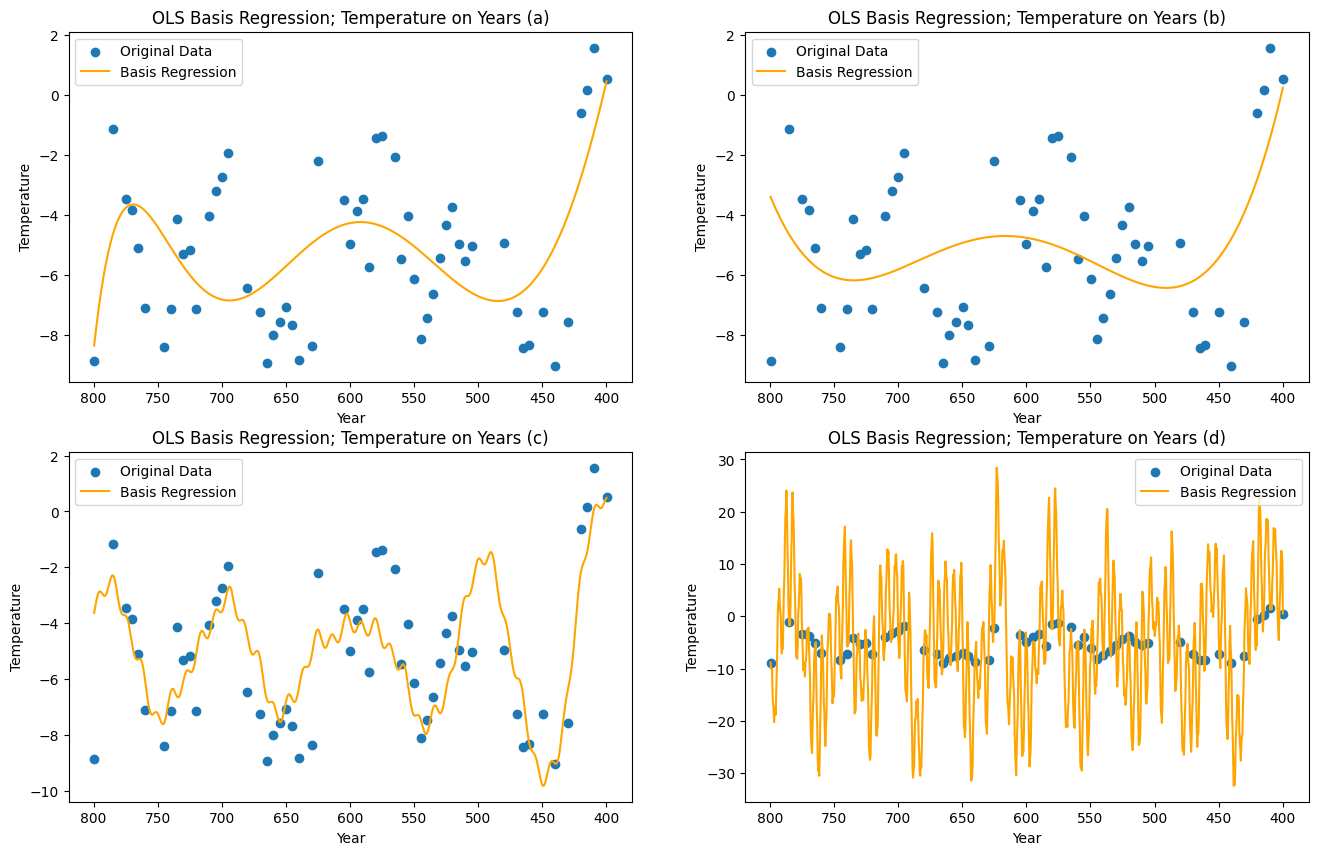
\includegraphics[width=0.80\linewidth]{output.png}
        \caption{Resulting Plot}
    \label{fig:enter-label}
\end{figure}

\bigskip
\textbf{2.}

\textbf{Part (a);}
 \begin{itemize}
     \item Train MSE: 4.82
     \item Test MSE: 7.96
 \end{itemize}


\textbf{Part (b);}
 \begin{itemize}
     \item Train MSE: 5.53
     \item Test MSE: 8.71
 \end{itemize}

\textbf{Part (c);}
 \begin{itemize}
     \item Train MSE: 2.88
     \item Test MSE: 5.97
 \end{itemize}


\textbf{Part (d);}

 \begin{itemize}
     \item Train MSE: 0.64
     \item Test MSE: 58.97
 \end{itemize}

(a) shows a moderate increase in MSE from training to test set, from 4.82 to 7.96. This might indicate a slight overfitting, as the model performs notably better on the training data than on unseen data, but the effect is relatively mild.

(b) also exhibits an increase in MSE from the training set to the test set, from 5.53 to 8.71. Similar to part (a), this suggests a slight overfitting, where the model fits the training data fairly well but generalizes with less accuracy to the test data.
  
(c) has training MSE of 2.88 and test MSE of 5.97. The pattern remains consistent with mild overfitting, where the model performs better on the training data than on the test data, although the gap between training and test MSE is larger than in parts (a) and (b), indicating a better fit on the training data.
  
(d) exhibits a dramatic difference, with a very low training MSE of 0.64 and a very high test MSE of 58.97. This is a clear indication of significant overfitting.

Parts (a), (b), and (c) exhibit signs of overfitting, with part (c) showing the best performance among them due to the lowest training MSE and a moderately low test MSE. However, the model in part (d) is the most overfitted, as evidenced by the vast disparity between its training and test MSE values. The exceptionally low training MSE in contrast to the extremely high test MSE suggests that the model captures the noise or idiosyncrasies in the training data rather than the underlying trend.

\bigskip
\textbf{3.}

The transforms \(f\) in basis function linear regression serve to scale input features, improving numerical stability and model flexibility. By adjusting the range of input values, these transforms mitigate computational issues like overflow or underflow, especially relevant for large-scale inputs such as years. Also, scaling facilitates the modeling of complex nonlinear relationships through basis functions (polynomial, exponential, trigonometric), enabling a linear regression framework to capture intricate data patterns effectively.

\bigskip
\textbf{4.}

The space complexity of linear regression primarily depends on the dimensionality of the feature space \(D\) after applying basis transformations, requiring \(O(ND)\) space to store the transformed training set \( \phi(\mathbf{X}) \). This is a departure from the simpler \(O(N)\) space requirement of kNN, which directly stores the training data without transformation. While the kernelized approach also stores the entire training set, it dynamically calculates kernel functions during prediction, avoiding the additional space needed for transformed features.\\

In terms of time complexity, linear regression's efficiency of predicting is high. Predictions involve a dot product between the weight vector \( \mathbf{w} \) and the transformed input \( \phi(x^*) \), scaling with \(O(D)\), making it relatively efficient, especially when \(D\) is not excessively large. This contrasts with the \(O(N)\) prediction complexity of both kNN and kernelized regression, where computations depend on the entire training set size, potentially making these methods slower for predictions in large datasets.

\bigskip
\textbf{5.}

kNN, with its reliance on the nearest neighbors, shows simplicity and effectiveness for data where proximity correlates strongly with outcomes, yet its performance decreases with increasing dataset size or dimensionality due to computational inefficiencies and dimensionality. Kernelized regression, utilizing kernel functions to encapsulate data similarities, showes its strength in modeling complex, nonlinear relationships without necessitating high-dimensional feature expansions, though at the expense of computational intensity and the nuanced selection of kernel parameters.Linear regression emerged as a versatile technique, combinig the interpretability of linear models with the capacity to approximate nonlinear phenomena through feature transformations. The empirical analysis across these regression techniques highlights no universally optimal solution; instead, the appropriateness of each method pivots on the dataset's nature, copmutation power, etc.

\end{solution}
% rewq

%%%%%%%%%%%%%%%%%%%%%%%%%%%%%%%%%%%%%%%%%%%%%
% Problem 5
%%%%%%%%%%%%%%%%%%%%%%%%%%%%%%%%%%%%%%%%%%%%%
\newpage
\begin{problem}[Deriving Linear Regression, 10pts]

  In the previous problems, you focused on implementing regressions
  and exploring their fits on data. Now we will turn to some more
  analytic work.  Specifically, the solution for the least squares
  linear regressions ``looks'' kind of like a ratio of covariance and
  variance terms.  In this problem, we will make that connection more
  explicit. \\

  \noindent Let us assume that our data are tuples of scalars $(x,y)$ that are
  described by some joint distribution $p(x,y)$.  For clarification, the joint distribution $p(x,y)$ is just another way of saying the ``joint PDF'' $f(x,y)$, which may be more familiar to those who have taken Stat 110, or equivalent. \\
  
  \noindent We will consider the process of fitting these data from this distribution with the best linear model
  possible, that is a linear model of the form $\hat{y} = wx$ that
  minimizes the expected squared loss $E_{x,y}[ ( y - \hat{y} )^2
  ]$.\\

\noindent \emph{Notes:} The notation $E_{x, y}$ indicates an
expectation taken over the joint distribution $p(x,y)$.  Since $x$ and
$y$ are scalars, $w$ is also a scalar.
  
  \begin{enumerate}

  \item Derive an expression for the optimal $w$, that is, the $w$
    that minimizes the expected squared loss above.  You should leave
    your answer in terms of moments of the distribution, e.g. terms
    like $E_x[x]$, $E_x[x^2]$, $E_y[y]$, $E_y[y^2]$, $E_{x,y}[xy]$
    etc.

\item Provide unbiased and consistent formulas to estimate $E_{x, y}[yx]$
 and $E_x[x^2]$ given observed data $\{(x_n,y_n)\}_{n=1}^N$.

\item In general, moment terms like $E_{x, y}[yx]$, $E_{x, y}[x^2]$,
  $E_{x, y}[yx^3]$, $E_{x, y}[\frac{x}{y}]$, etc. can easily be
  estimated from the data (like you did above).  If you substitute in
  these empirical moments, how does your expression for the optimal
  $w^*$ in this problem compare with the optimal $w^*$ that we see in
  Section 2.6 of the cs181-textbook?

\item Many common probabilistic linear regression models assume that
  variables x and y are jointly Gaussian.  Did any of your above
  derivations rely on the assumption that x and y are jointly
  Gaussian?  Why or why not?
    
\end{enumerate}
  
\end{problem}

\begin{solution}

\bigskip
\textbf{1.}

Expanding the squared term and taking the expectation gives:
$$
E_{x, y}[(y - wx)^2] = E_{x, y}[y^2 - 2wxy + w^2x^2]
$$

which can be broken down into:
$$
E_{x, y}[y^2] - 2wE_{x, y}[xy] + w^2E_{x, y}[x^2]
$$

To find the \(w\) that minimizes this expression, we take the derivative with respect to \(w\) and set it to zero:
$$
\frac{d}{dw}(E_{x, y}[y^2] - 2wE_{x, y}[xy] + w^2E_{x, y}[x^2]) = 0
$$

Simplifying, we get:
$$
-2E_{x, y}[xy] + 2wE_{x, y}[x^2] = 0
$$

Solving for \(w\), we find:
$$
w = \frac{E_{x, y}[xy]}{E_{x, y}[x^2]}
$$

We find that optimal \(w\) that minimizes the expected squared loss for a linear model \(\hat{y} = wx\) under the joint distribution \(p(x, y)\) is given by the ratio of the covariance of \(x\) and \(y\) to the variance of \(x\), which makes sense with the intuition that the slope in a linear regression model reflects how much \(y\) changes with \(x\), normalized by the variability in \(x\).


\bigskip
\textbf{2.}

\textbf{Estimating \(E_{x, y}[yx]\)
}

The expected value \(E_{x, y}[yx]\) can be estimated by the sample mean of the product of \(x\) and \(y\) for all observed pairs. The unbiased and consistent estimator for \(E_{x, y}[yx]\) is given by:

$$
\hat{E}_{x, y}[yx] = \frac{1}{N} \sum_{n=1}^N x_n y_n
$$

\textbf{Estimating \(E_x[x^2]\)
}

Similarly, the expected value \(E_x[x^2]\) represents the second moment about the origin for \(x\). It can be estimated from the data as:

$$
\hat{E}_x[x^2] = \frac{1}{N} \sum_{n=1}^N x_n^2
$$

This is the sample mean of the squared values of \(x\), providing an unbiased and consistent estimate of \(E_x[x^2]\).

\bigskip
\textbf{3.}

The textbook formula is for a more general case where \(\mathbf{X}\) is a design matrix with multiple features for each observation, and \(\mathbf{w}^*\) is a vector of weights. The formula given is:

$$
\mathbf{w}^* = (\mathbf{X}^\top \mathbf{X})^{-1} \mathbf{X}^\top \mathbf{y}
$$

The key difference is in the dimensionality of the problem. The expression for \(w\) in the simple linear regression case is scalar, focusing on a single predictor variable \(x\) and a single response variable \(y\). however, the \(\mathbf{w}^*\) from the textbook accounts for multiple predictors for each observation.
When we  substitute empirical moments into the simple linear regression formula, we're essentially using specific instances of the more general matrix operations. Basically, the formula for \(\mathbf{w}^*\) generalizes the concept of finding the optimal weights to multiple dimensions. If we were to consider the simple linear regression scenario as a special case of the multiple regression, the matrix formula would yield the same insight as the scalar formula derived from empirical moments: the weight vector minimizes the squared error loss between the predicted and actual values.

\bigskip
\textbf{4.}

The derivations do not explicitly rely on the assumption that \(x\) and \(y\) are jointly Gaussian.

The formula for the optimal \(w\),
   $$
   w = \frac{E_{x, y}[xy]}{E_{x, y}[x^2]},
   $$
was derived based on minimizing the expected squared loss, \(E_{x, y}[(y - wx)^2]\), without making any specific assumptions about the distribution of \(x\) and \(y\). This derivation is purely algebraic and relies on the properties of expectations and does not necessitate any particular distributional form for \(x\) and \(y\). The formulas to estimate \(E_{x, y}[yx]\) and \(E_x[x^2]\) from observed data,
   $$
   \hat{E}_{x, y}[yx] = \frac{1}{N} \sum_{n=1}^N x_n y_n
   $$
   and
   $$
   \hat{E}_x[x^2] = \frac{1}{N} \sum_{n=1}^N x_n^2,
   $$
are based on the sample means of products and squares of the observed values. These estimations are standard procedures that do not assume any specific distribution for \(x\) and \(y\); they are applicable as long as the law of large numbers holds, which does not require \(x\) and \(y\) to be jointly Gaussian.
While the derivations did not assume a joint Gaussian distribution, many probabilistic linear regression models do make this assumption because Gaussian distributions has desirable properties, such as being fully described by their mean and variance, and the linear transformations of Gaussian variables are also Gaussian, which simplifies analysis. Also, under certain conditions, averages of random variables converge in distribution to a Gaussian, even whn the original variables themselves are not Gaussian. This makes the Gaussian assumption reasonable for a wide range of applications.

\end{solution}

%%%%%%%%%%%%%%%%%%%%%%%%%%%%%%%%%%%%%%%%%%%%%
% Name and Calibration
%%%%%%%%%%%%%%%%%%%%%%%%%%%%%%%%%%%%%%%%%%%%%
\newpage
\subsection*{Name}

\subsection*{Collaborators and Resources}
Whom did you work with, and did you use any resources beyond cs181-textbook and your notes?

\begin{itemize}
    \item Wikipedia
    \item Stat111 textbook
\end{itemize}

\end{document}
